
\documentclass{abgabe}

\begin{document}
\begin{questions}
    \qformat{\thequestion. \textbf{\thequestiontitle} \hfill}
    \titledquestion{Builder Pattern}

    In der Vorlesung wurde das Builder Pattern \emph{nicht} vorgestellt.

    \begin{parts}
        \part
        Erklären Sie mit eigenen Worten, welchen Nutzen das Builder Pattern bringt und wo die typischen Einsatzgebiete liegen.

        \begin{solution}
            StackOverflow-Nutzer \href{https://stackoverflow.com/a/55749042/9055591}{Hoopjie} fasst es sehr gut zusammen:
            \begin{displayquote}
                Using a builder pattern has a few advantages:

                \begin{enumerate}
                    \item Unlike with setters (which make your class mutable), a builder can be used to contruct immutable objects. In many cases immutable objects are preferred over mutable objects, because they are easier to understand and maintain, and because they avoid the need for locking in multithreaded environments.
                    \item A builder can make sure that the object satisfies some invariants even directly after construction. For example, if your class has a \texttt{name} field which must never be null, the builder can check this condition and fail to construct the object when not satisfied.
                \end{enumerate}

                Both things you can also accomplish by using a constructor which takes all the class contents as parameters, but that will be quite unreadable when your class has more than a few fields to initialize.

            \end{displayquote}
        \end{solution}

        \newpage
        \part
        Finden Sie ein geeignetes Beispiel und erklären Sie dieses.
        Modellieren (Klassendiagramm) und \emph{implementieren} Sie für diesen Anwendungsfall das Builder Pattern.

        \begin{solution}
            \begin{center}
                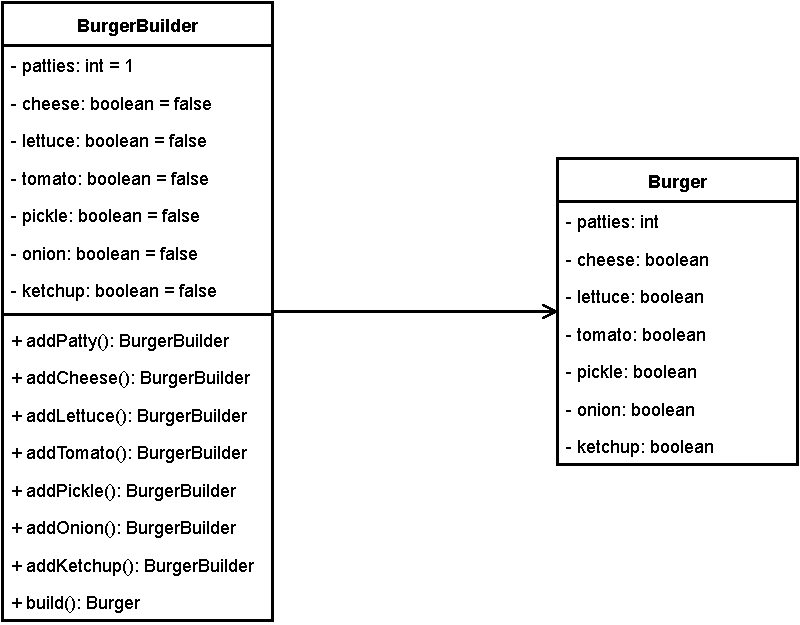
\includegraphics[width=.75\textwidth]{swt_h09_burger.pdf}
            \end{center}

            Der dazugehörige Code befindet sich im Anhang.
        \end{solution}
    \end{parts}
\end{questions}

\end{document}